\documentclass[10pt]{article}

\usepackage{spheric}
%%%TITLE
\title{SPH energy balance during the generation and propagation of gravity waves}
\date{}

%%AFFILIATIONS
\author[1]{Domenico Davide MERINGOLO$^\dagger$}
\author[1]{Yong LIU}
\author[2]{Andrea COLAGROSSI}
\affil[1]{Ocean University of China, Qingdao, 266100}
\affil[2]{CNR-INSEAN, Rome, 00128, Italy}

\affil[$\relax$]{\email{\dagger}{davide.m86@gmail.com}}


%%DOCUMENT
\begin{document}

\maketitle

%\SelectedTopics{}

%%PLEASE PUT YOUR ABSTRACT HERE
\begin{abstract}
Recently, different works regarding the energy conservation properties of the SPH model have been presented. For example, Antuono et al. \cite{antuono2015energy} analyzed the energy balance in the SPH scheme when a diffusive correction is used in the continuity equation for improving the stability of the scheme. In Cercos-Pita et al. \cite{cercos2017sph} the energy conservation analysis has been extended to the case of moving solid boundaries when the flow is dominated by the viscous effects. In the present work, a further investigation on the energy conservation is discussed for problems where moving solid boundaries interact with an inviscid flow. The solid boundary techniques adopted are: the ghost and the fixed ghost particles. A first problem in which the dynamic is generated by a water patch falling into a still water tank is analyzed. In this case, the dissipation processes due to the diffusive and viscous numerical corrections are investigated. Then, a problem of relevant interest in coastal engineering field, concerning the wave generation and propagation in a wave flume, is studied. Two limit cases are analyzed, the first one is a wave flume with a flat bottom and a vertical wall, representative of a wave reflective condition (Fig. \ref{fig:43-1}a), while the second one is a sloping bottom flume, representative of a wave absorbing condition (Fig. \ref{fig:43-1}b).
\begin{figure}[!htb]
\centering
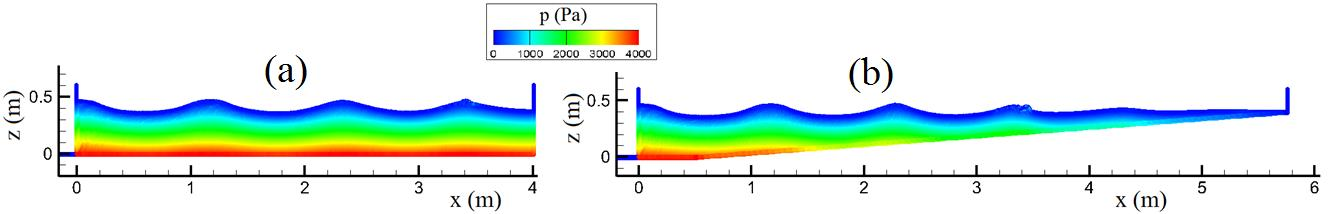
\includegraphics[width=0.95\textwidth]{43-1.png}
\caption{Waves propagation with pressure field for the analyzed cases: in (a) is the wave reflective condition,
while in (b) is the wave absorbing one.}\label{fig:43-1} 
\end{figure}

\begin{figure}[!htb]
\centering
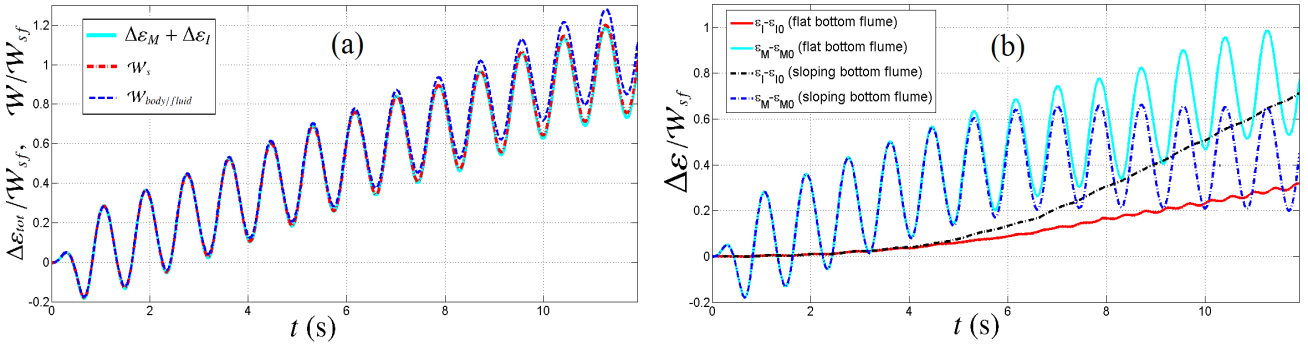
\includegraphics[width=0.95\textwidth]{43-2.png}
\caption{(a) Nominal work, $W_\text{body/fluid}$, effective work, $W_S$, made by the solid boundaries in comparison with the total energy evaluated inside the fluid domain, $\Delta\varepsilon_M + \Delta\varepsilon_I$. (b) Comparison of mechanical and internal energies variations for the flat and sloping bottom flume.}\label{fig:43-2} 
\end{figure}
The wave generation is studied considering the work made by the solid boundary on the fluid mass. The nominal work, $W_\text{solid/fluid}$, and actual work, W S , are analyzed through a convergence analysis, showing that when the spatial resolution is increased $W_S\rightarrow W_\text{solid/fluid}$. These results are presented in Fig. \ref{fig:43-2}a, in which it is possible to see that, according with the second law of thermodynamics, $W_S$ equals the variation of total energy (mechanical+internal) evaluated inside the fluid domain $\Delta\varepsilon_{tot}=\Delta\varepsilon_M + \Delta\varepsilon_I$ (being $\Delta\varepsilon=\varepsilon-\varepsilon_0$ with $\varepsilon_0$ the initial energy), while at the same time it underestimates the nominal work performed by the wave-maker. Successively, the dynamics of the wave propagation is analysed from an energy viewpoint, by inspecting the single energy components, namely the potential, kinetic, compressible and numerical-dissipated energies, evaluated inside the fluid domain. Fig. \ref{fig:43-2}b presents the comparison of the time evolution of mechanical, $\Delta\varepsilon_M$, and internal energies, $\Delta\varepsilon_I$, for the reflective and non-reflective cases. Because of the development of breaking waves, in the latter case the mechanical energy reaches quickly a stable condition with oscillations around a constant value.



\end{abstract}


%%THE END OF ABSTRACT

\addbib

\end{document}
